\documentclass[a4paper,12pt]{article}
\usepackage[utf8]{inputenc}
\usepackage[T2A]{fontenc}
\usepackage[english, russian]{babel}
\usepackage{amsthm}
\usepackage{amsmath}
\usepackage{amssymb}
\usepackage{tikz}
\usepackage{textcomp}
\usepackage{esint}
\usepackage[unicode]{hyperref}
\usepackage{indentfirst}
\usepackage{algorithm}
\usepackage[noend]{algpseudocode}
\usepackage{amsmath,amsfonts,amssymb,amsthm,mathtools}
\usetikzlibrary{positioning,arrows}
\usepackage{graphicx}
\setlength{\topmargin}{-0.5in}
\setlength{\textheight}{9.1in}
\setlength{\oddsidemargin}{-0.4in}
\setlength{\evensidemargin}{-0.4in}
\setlength{\textwidth}{7in}
\setlength{\parindent}{0ex}
\setlength{\parskip}{1ex}
\usepackage{siunitx}

\usepackage{multicol}
\usetikzlibrary{trees}
\usepackage{fancyhdr}
\usepackage{gensymb}

\newcommand{\bbR}{\mathbb R}
\newcommand{\eps}{\varepsilon}
\newcommand{\bbN}{\mathbb N}
\newcommand{\dif}{\mathrm{d}}

\pagestyle{fancy}
\makeatletter
\fancyhead[L]{}

\fancyfoot[R]{\thepage}
\fancyfoot[C]{}

\renewcommand{\maketitle}{
	\noindent{\bfseries\scshape\large\@title\ \mdseries\upshape}\par
	\noindent {\large\itshape\@author}
	\vskip 2ex}
\makeatother




\begin{document}
	
\Large \textbf { \begin{center}
		Работа 10.1\\ Электронный парамагнитный резонанс \\
		Селюгин Михаил, 876 \\
\end{center}}


	\section{Теория вопроса}
		Энергетический уровень электрона в присутствии магнитного поля $B$ расщепляется на два подуровня, расстояние между которыми равно:
		\begin{equation}
		    \Delta E = E_2 - E_1 = 2\mu B
		\end{equation}
		Резонансное значение частоты:
		\begin{equation}
		    \hbar\omega_0 = \Delta E =2\mu B
		\end{equation}
	    При переходе с нижнего на верхний уровень квант энергии поглощается, а при обратном переходе излучается квант той же частоты. Возбуждение электронных резонансных переходов электромагнитным полем с частотой $\omega_0$ носит название <<электронного парамагнитного резонанса>>
	    
	    Сигнал ЭПР наблюдается на неспаренных электронах. В работе используется образец свободного радикала ДФПГ.
	    
	    \begin{figure}[h!]
			\centering
			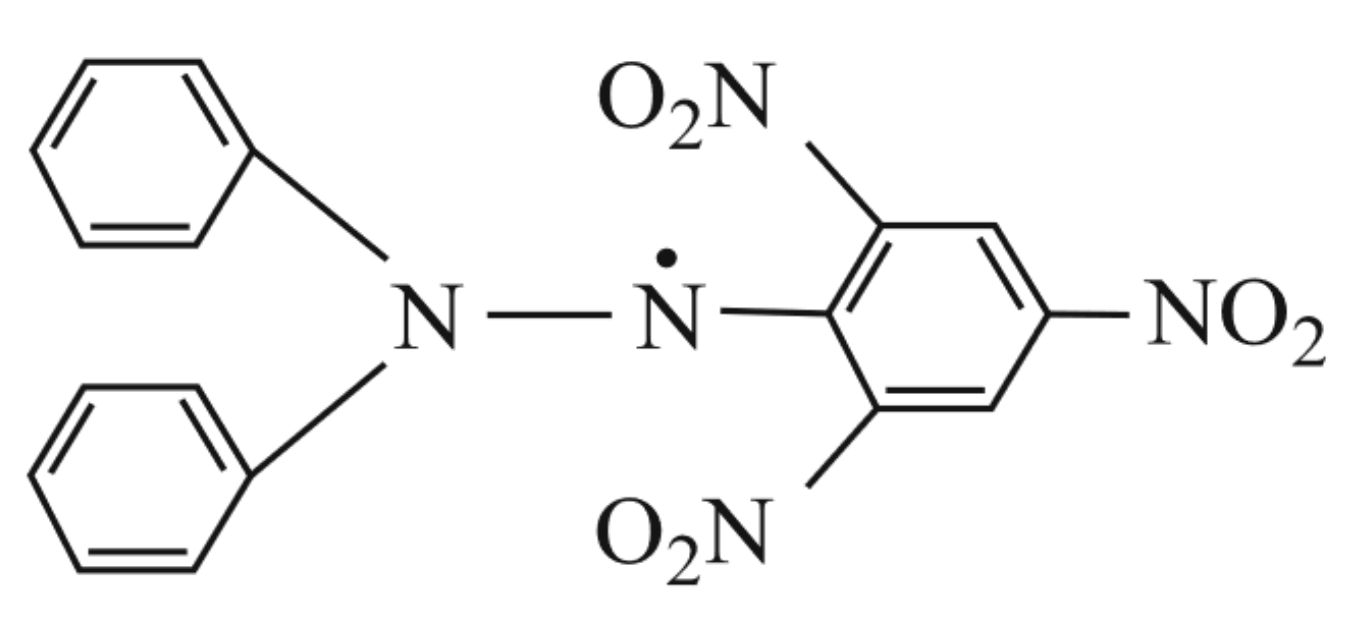
\includegraphics[width=0.5\linewidth]{dfpg}
			\caption{Дифенилпикрилгидразил}
		\end{figure}
	
    Рассмотрим основные процессы, влияющие на ширину линии ЭПР. В отсутсвие высокочастотного поля заселенность верхнего и нижнего уровней $N_u$ и $N_d$ определяется температурой и описывается формулой Больцмана.
    \begin{equation}
        \frac{N_u}{N_d} = exp\left(-\frac{\Delta E}{kT}\right)
    \end{equation}
    В присутствии резонансного поля между уровнями возникают индуцированные переходы, ведущие к тому, что заселенность верхнего уровня растет, а нижнего падает. Восстановление теплового равновесия происходит двумя способами: спин-спиновой и спин-решеточной релаксацией.
    Отличить их друг от друга можно по температурной зависимости: спин-решеточное взаимодействие быстро возрастает с температурой(числом фононов), спин-спиновое от температуры практически не зависит.
    
    Согласно соотношению неопределенностей:
    \begin{equation}
       \Delta E \tau \simeq \hbar \Delta\omega\tau \simeq 1
    \end{equation}
	
        В работе требуется получить ЭПР сигнал на ДФПГ. Известно, что связь между магнитным моментом электрона и его механическим моментом выражается через гиромагнитное соотношение:
        \begin{equation}
            \bf{\mu} = \gamma\bf{M}
        \end{equation}
        Если магнитный момент выражается в магнетонах Бора, а механический в единицах $\hbar$, то связь выражается через фактор Ланде:
        \begin{equation}
            \frac{\bf{\mu}}{\mu_B} = \frac{g\bf{M}}{\hbar}
        \end{equation}
        \newline
        Эта формула справедлива и для проекций. Можно выразить $g$-фактор через определяемые экспериментально величины:
        \begin{equation}
            g = \frac{\hbar\omega_0}{\mu_B B}
        \end{equation}
        Эксперимент выполняется с помощью спектроскопа.
        \begin{figure}[h!]
			\centering
			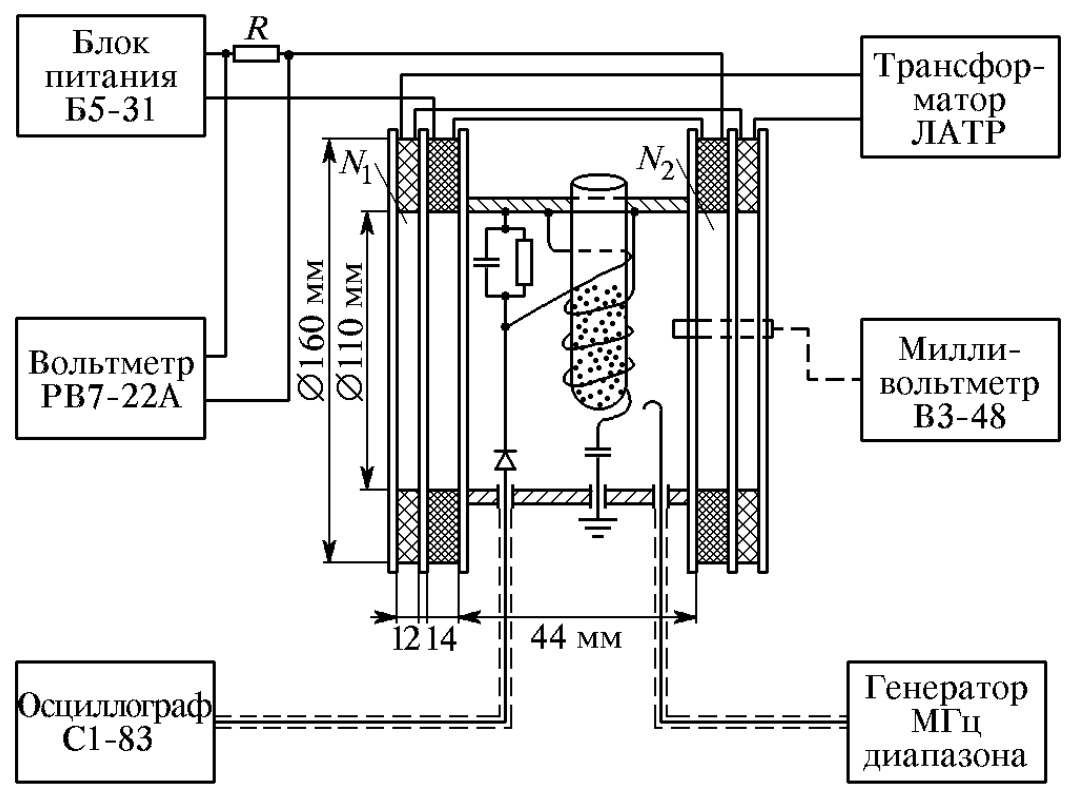
\includegraphics[width=0.7\linewidth]{exp}
			\caption{Блок-схема установки для наблюдения ЭПР в молекуле ДФПГ}
		\end{figure}        
		
		Параметры установки: $N_1 = 5850, N_2 = 1260$
		
    \newpage
    \section{Результаты измерений}
    
	\begin{enumerate}
		\item[I.] Измерение $g$-фактора электрона.
		\begin{itemize}
			\item Значение резонансной частоты измерено по лимбу генератора: $\omega_{0} = 167.7$ МГц.
			\item Параметры катушки, создающей постоянное магнитное поле: $N_{1} = 5850$, $N_{2} = 1260$.
			
			\item Параметры пробной катушки: $d = 14.9\pm 0.1$ мм, $n = N = 44$ витка.
			
			\item Угловая частота переменного тока: $\omega = 2$ кГц.
			
			\item Значение постоянного тока в катушке: $U = 184.3$ мВ.
			
			\item Показания лампового милливольтметра: $V = 15.6$ мВ.
			
		\end{itemize}
	
	\item[II.] Определение ширины линии ЭПР.
		
		\begin{itemize}
			\item Амплитуда модулирующего поля: $A_{\text{полн.}} = 9$ дел.
			
			\item Ширина кривой резонансного поглощения на полувысоте: $A_{1/2} = 0.8$ дел.
			
			\item ЭДС индукции в пробной катушке: $\mathcal{E}_{i} = 11.2$ мВ.
			
		\end{itemize}
		 
		На осциллографе наблюдается кривая резонсного поглощения :
		\begin{figure}[ht]
			\centering
			\caption{Наблюдаемая с помощью осциллографа линия резонансного поглощения в кристалле ДФПГ}
			\label{pic2}
			\includegraphics[]{photo.jpg}
		\end{figure}
	\end{enumerate}

	\newpage
	
	\section{Обработка результатов}
	
	\begin{enumerate}
		\item[I.] Оценим $g$ фактор электрона. Для этого с помощью пробной катушки определим индукцию магнитного поля пиз формулы:
		
		\begin{equation}
		V = nB_{0}S\omega = \frac{\pi}{4}nB_{0}d^{2}\omega \Longrightarrow B_{0} = \frac{4V}{\pi nd^{2}\omega}.
		\end{equation}
		
		Получим результат:
		\[B_{0} \approx 1.02\text{ мТл}.\]
		
		Рассчитаем погрешность:
		$$\varepsilon_{d} \approx 0.6\%,\ \varepsilon_{V}\approx 0.5\%\ \Rightarrow \varepsilon_{B_{0}} = \sqrt{2\varepsilon_{d}^{2} + \varepsilon_{V}^{2}} = 1.0\%.$$
		Таким образом: 
		\[B_{0} = 1.02\pm 0.01 \text{ мТл } (\varepsilon\approx 1\%).\]
		
		Вычислим $g$-фактор:
		\[g = \frac{\hbar\omega_{0}}{\mu_{\text{Б}}} \]
		
		\[g =\approx 1.87.\]
		
		Рассчитаем погрешность: $$\varepsilon_{B_{0}} = 1.0\%,\ \varepsilon_{\omega_{0}}\approx 0.6\%\ \Rightarrow \varepsilon_{g} = \sqrt{\varepsilon_{\omega_{0}}^{2}+\varepsilon_{B_{0}}^{2}}\approx 1.2\%.$$
		Значит:
		\[g = 1.87\pm 0.02.\]
		
		\item[II.] Оценим ширину линии ЭПР.
		
		Определим амплитуду моделирующего поля по формуле:
		\begin{equation}
		B_{\text{мод.}} = \sqrt{2}\frac{2\mathcal{E}_{i}}{\pi^{2}d^{2}n\nu},
		\end{equation}
		где $\nu = 400$ Гц -- частота модулирующего напряжения.
		
		Тогда:
		\[B_{\text{мод.}} \approx 0.82\text{ мТл.}\]
		Погрешность: 
		$$\varepsilon_{d} = 0.7\%,\  \varepsilon_{\mathcal{E}_{i}} = 0.9\% \Rightarrow \varepsilon_{B_{\text{мод.}}} = \sqrt{2\varepsilon_{d} + \varepsilon_{\mathcal{E}_{i}}}\approx 1.3\%.$$ 
		Значит
		\[B_{\text{мод.}} = 0.82\pm 0.01\text{ мТл } (\varepsilon = 1,3\%).\]
		
		Далее определим полуширину линии ЭПР
		\begin{equation}
		\Delta B = \frac{A_{1/2}}{A_\text{полн.}}B_{\text{мод.}}.
		\end{equation}
		Значит полуширина на полувысоте линии резонансного поглощения равняется :
		\[\Delta B \approx 0.071\text{ мТл } = 0.71\text{ Гс}.\]
		
	Рассчет погрешности: $\varepsilon_{B_{\text{мод.}}} = 1,3\%$, $\varepsilon_{A_{\text{полн.}}} = \frac{0.05}{9}\approx 0.5\%$, $\varepsilon_{A_{1/2}} = \frac{0.05}{0.8}\approx 6.3\%$. Тогда 
	$$\varepsilon_{\Delta B} = \sqrt{\varepsilon_{A_{\text{полн.}}}^{2}+\varepsilon_{A_{1/2}}^{2}+\varepsilon_{B_{\text{мод.}}}^{2}}\approx 6.5\%.$$
	Получаем результат:
	\[\Delta B = 0.71\pm 0.05\text{ Гс } (\varepsilon = 6.5\%).\]
	\end{enumerate}

\section {Вывод}
	В ходе эксперимента было исследовано явление ЭПР на молекуле ДФПГ и получены значения $g$ фактора и полуширины линии ЭПР. При этом результаты оказались близки к табличным. Так, для $g$ фактора $g_{\text{изм}} = 1.87\pm 0.02, g_{\text{табл}} = 2 $. А для полуширины линии $\Delta B_{\text{изм}} = 0.71\pm 0.05\text{ Гс }, \Delta B_{\text{табл}}  \approx 1$. 


\end{document}


